\section{Experiments}
\label{experiments}

We illustrate the foregoing results on the hexarotor example from Section \ref{motivatingExample}.
Recall that we found the control performance, as measured by $J$ of Eq.??, to degrade as the robot's speed was increased.
We implemented the RAMPC controller of Section \ref{controlProblem}, and used the error-delay curves of Section \ref{delayErrorCurve}.

For the same sequence of increasing speeds (which translates to more stringent control demands), RAMPC performs better than MPC as illustrated in Fig.\ref{fig:RAMPCcost}.
\begin{figure}[t]
	\centering
	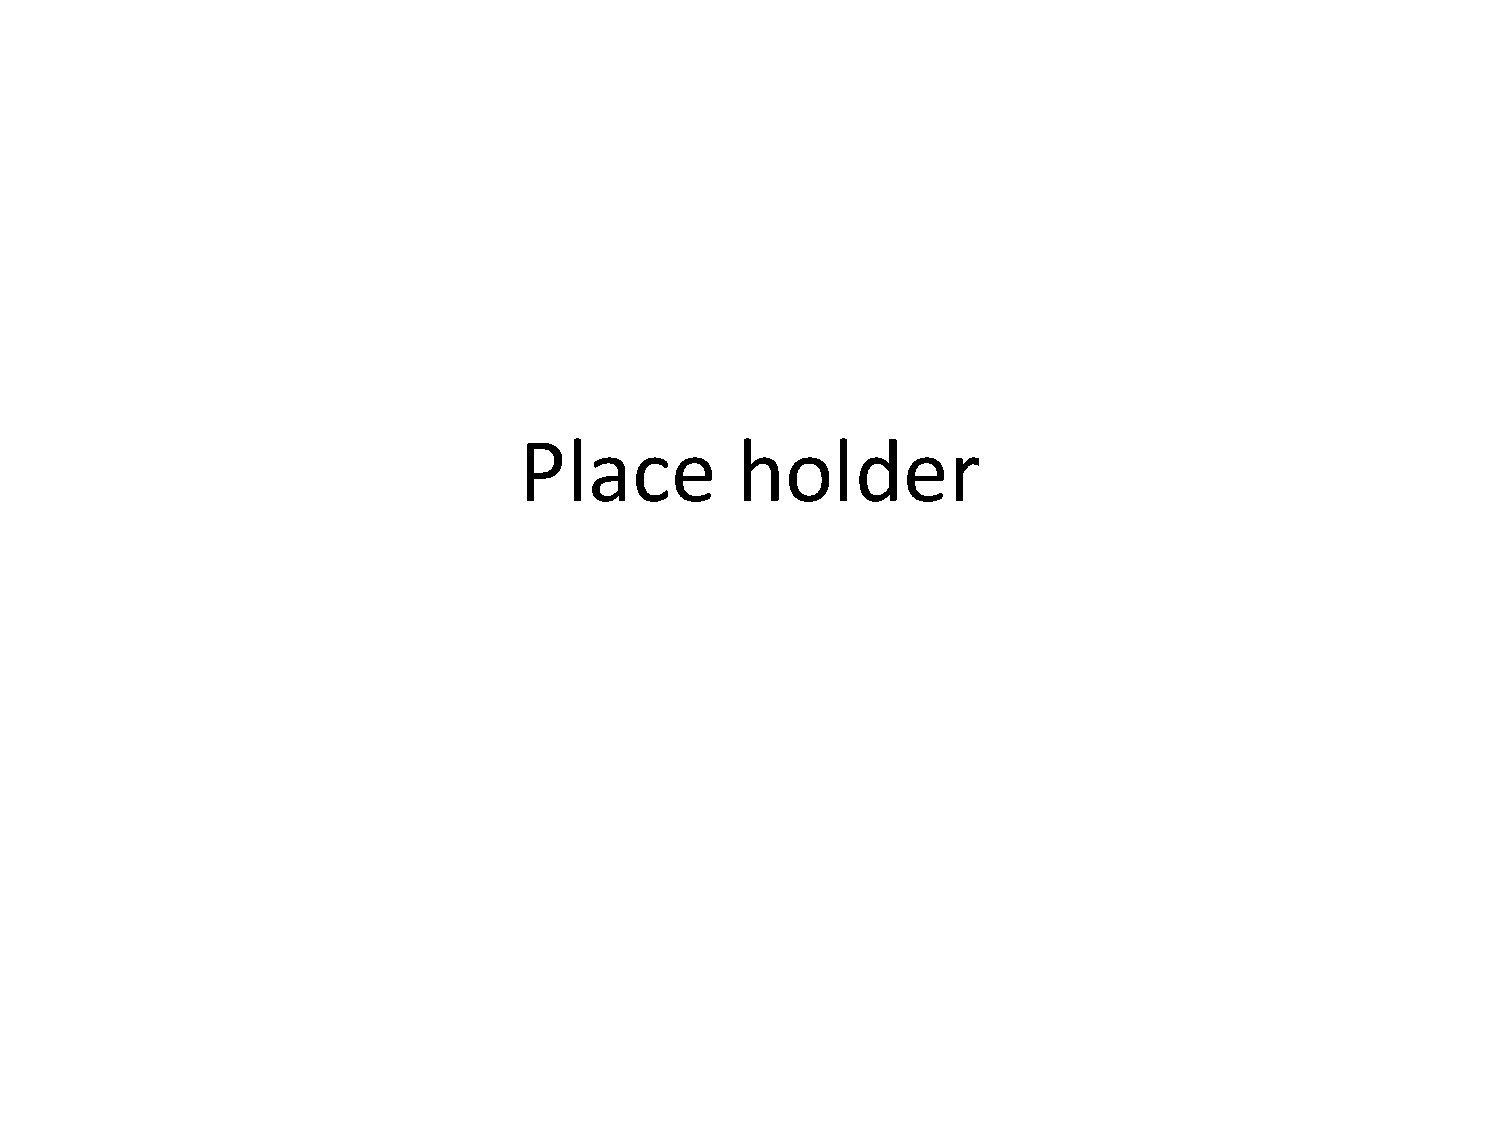
\includegraphics[width=0.7\linewidth]{figures/placeHolder}
	\caption{Cost function of RAMPC.}
	\label{fig:RAMPCcost}
\end{figure}

Fig.~\ref{fig:RAMPCtrajectory} shows the reference and actual trajectories of the hexarotor under RAMPC control.
\begin{figure}[t]
	\centering
	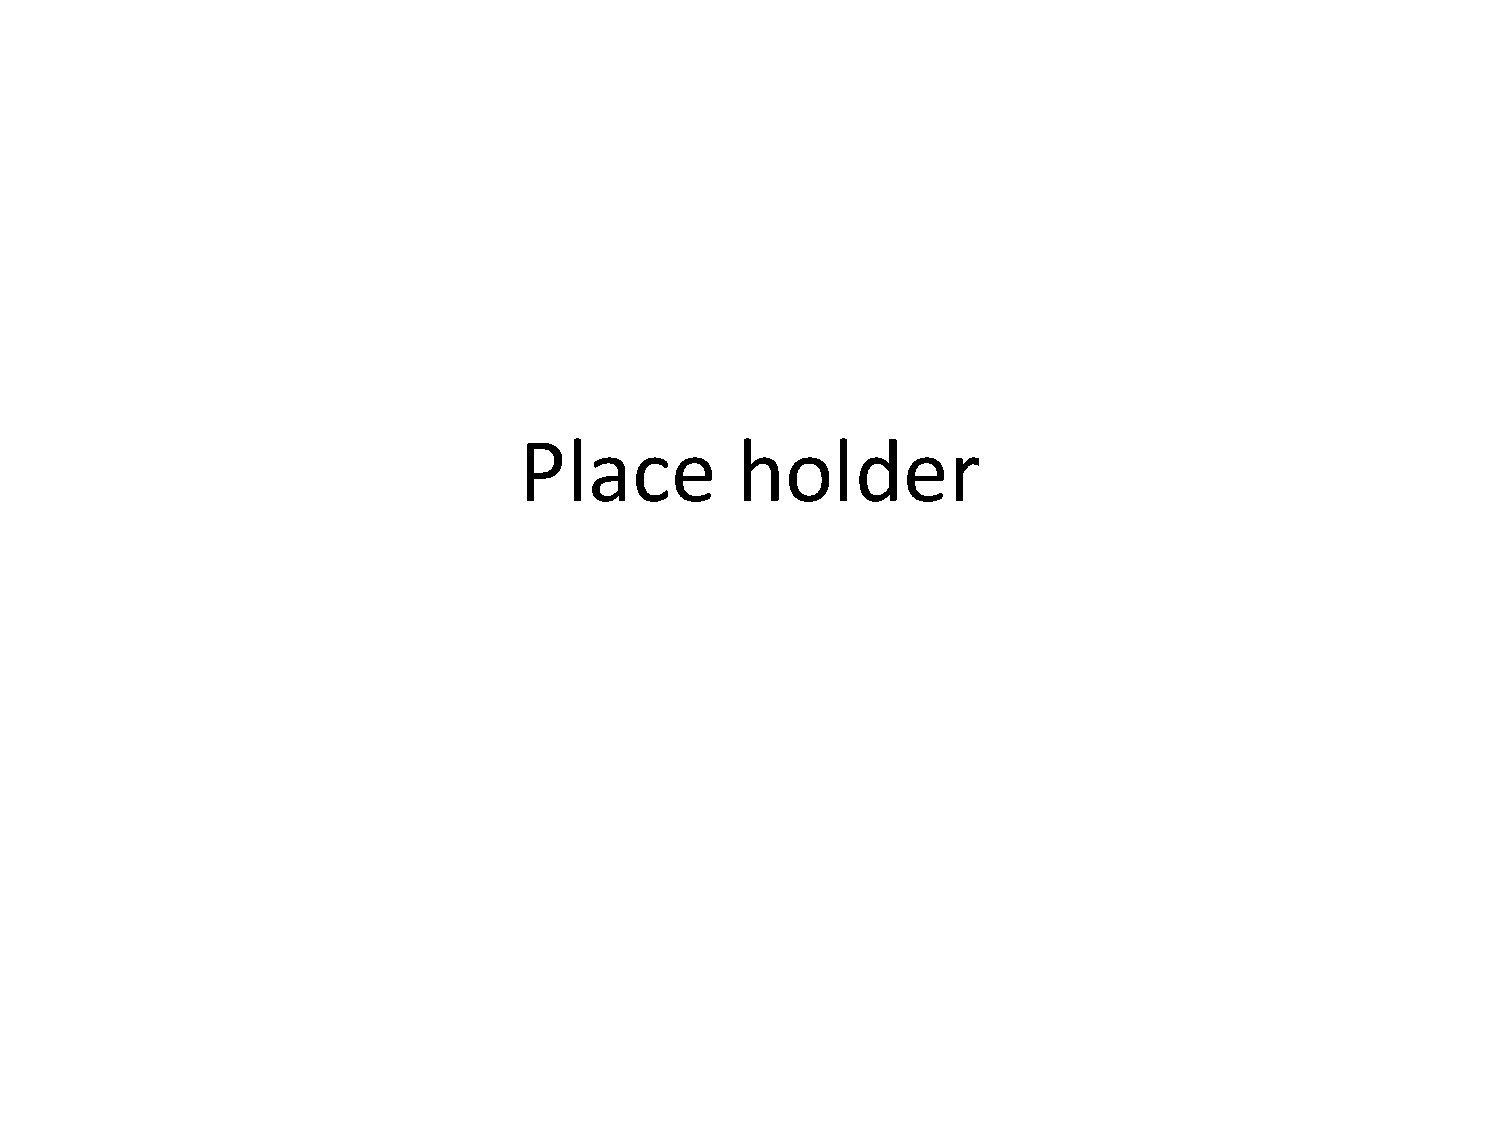
\includegraphics[width=0.7\linewidth]{figures/placeHolder}
	\caption{Reference and actual hexarotor trajectories controlled by RAMPC.}
	\label{fig:RAMPCtrajectory}
\end{figure}

Fig.~\ref{fig:modeSwitching} shows that the RAMPC indeed chooses different modes, indicating that awareness of the error/delay trade-off does lead to improved performance.
\begin{figure}[t]
	\centering
	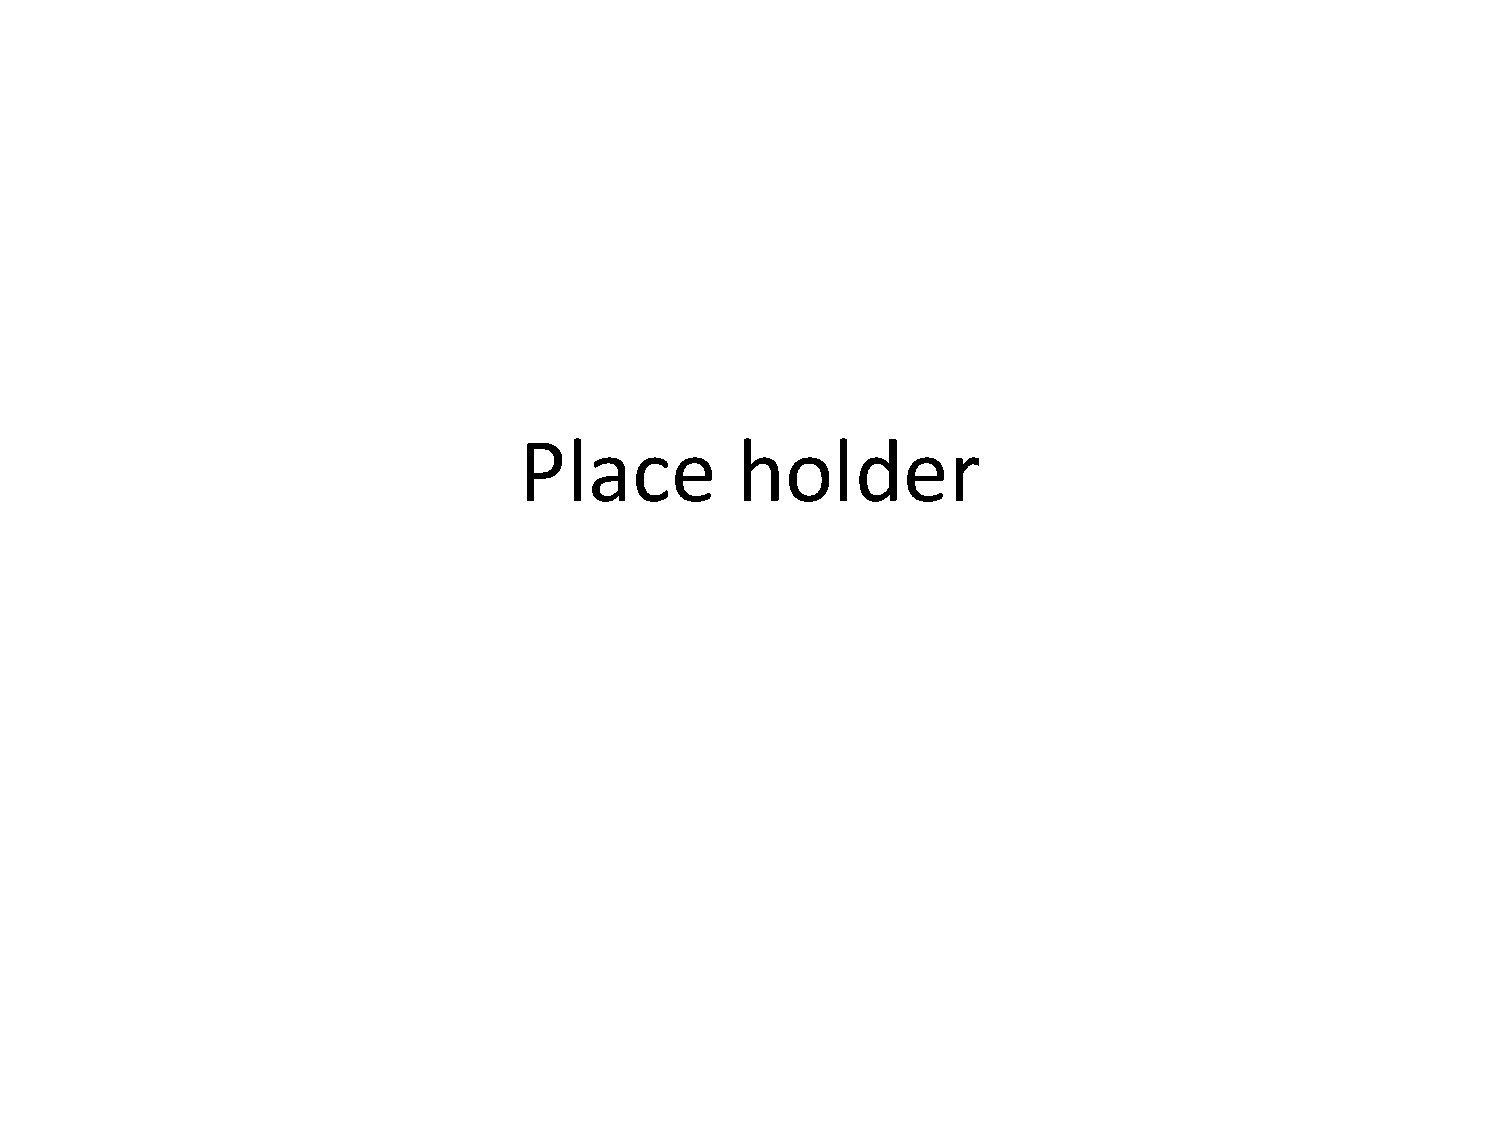
\includegraphics[width=0.7\linewidth]{figures/placeHolder}
	\caption{Mode switches of RAMPC.}
	\label{fig:modeSwitching}
\end{figure}